% ! TeX root = ../../main.tex
\chapter{Implementazione}
In questo capitolo vengono trattate le implementazioni e i pattern utilizzati per raggiungere i requisiti di progettazione presentati nel capitolo precedente. Sono presentate le effettive schermate ottenute partendo dai mockup mostrandone porzioni di codice particolarmente interessanti o dove sono stati applicati pattern.

\section{Organizzazione progetto}
I file del progetto sorgente sono organizzati in cartelle relative a ciascuna schermata, componente o funzionalità. L'albero delle cartelle viene presentato nel listato \ref{lst:projectDir} dove vengono espanse solo le cartelle di primo livello (model, views e dataProvider). All'interno della cartella \texttt{model} sono state inserite le classi che definiscono il modello dei dati utente (file \texttt{share\_data\_model.dart}) e i metodi/classi/interfacce di utilità (file \texttt{obj2map.dart}), in \texttt{views} sono presenti i file delle schermate raccolti in cartelle e infine in \texttt{dataProvider} sono contenuti tutti i provider di dati utilizzati dal \texttt{DataManager} (file \texttt{data\_manager.dart}) per il reperimento delle informazioni.

\begin{lstlisting}[language=C, caption={Albero della directory del progetto TotemBoschettoAR}, label={lst:projectDir}]
    TotemBoschettoAR/
        |
        +- model/
            |
            +- obj2map.dart
            +- share_data_model.dart
        +- views/
            |
            +- common/
            +- navigation_menu/
            +- home_page/
            +- stats_page/
            +- chart_page/
            +- info_page/
            +- home_page.dart
            +- stats_page.dart
            +- chart_page.dart
            +- info_page.dart
        +- dataProvider/
            |
            +- firebase_provider.dart
        +- unit_converter.dart
        +- data_manager.dart
        +- main.dart
\end{lstlisting}

\section{App Mobile}
Seguendo i mockup sono state sviluppate le diverse schermate per la condivisione dei progressi. Sono state effettuate alcune modifiche come si può notare dagli screenshot in figura \ref{fig:shareDataApp}: in sostituzione al nickname utente impostato è stata messa una breve indicazione, che si trovava precedentemente nella pagina di scansione, sul come visualizzare il QR code del totem e infine la schermata di caricamento è stata modificata sostituendo l'icona e mostrando un testo che informi l'utente del caricamento dei dati.
\begin{figure}[h!]
    \centering
    \subfloat[Pagina di condivisone progressi]{
        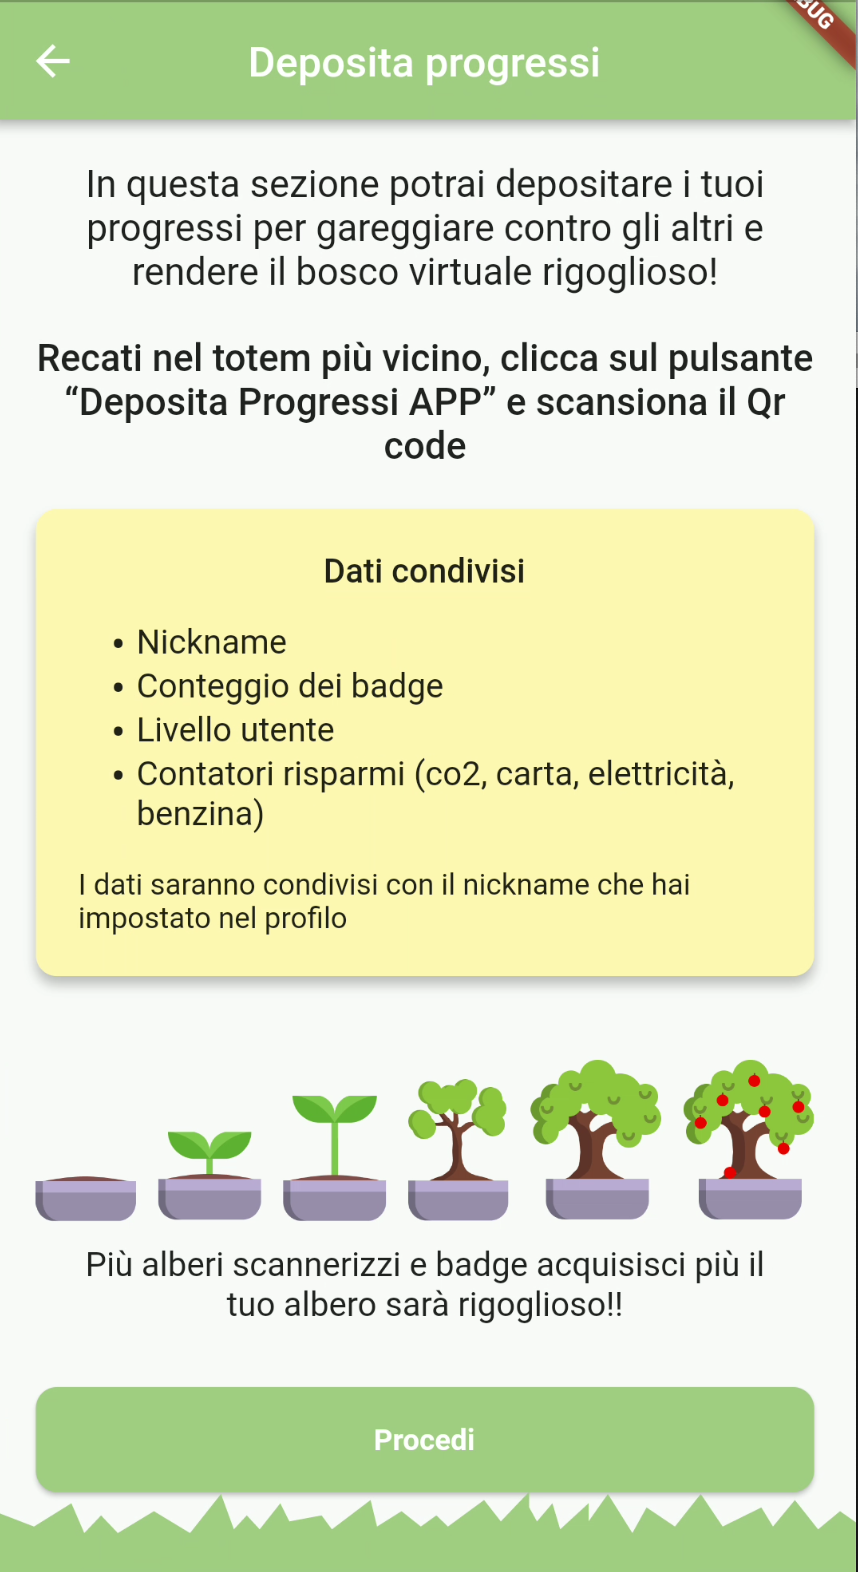
\includegraphics[width=0.3\textwidth]{img/app/uploadPage.png}
        \label{fig:sharePage}
    }
    \subfloat[Scansione QR code totem]{
        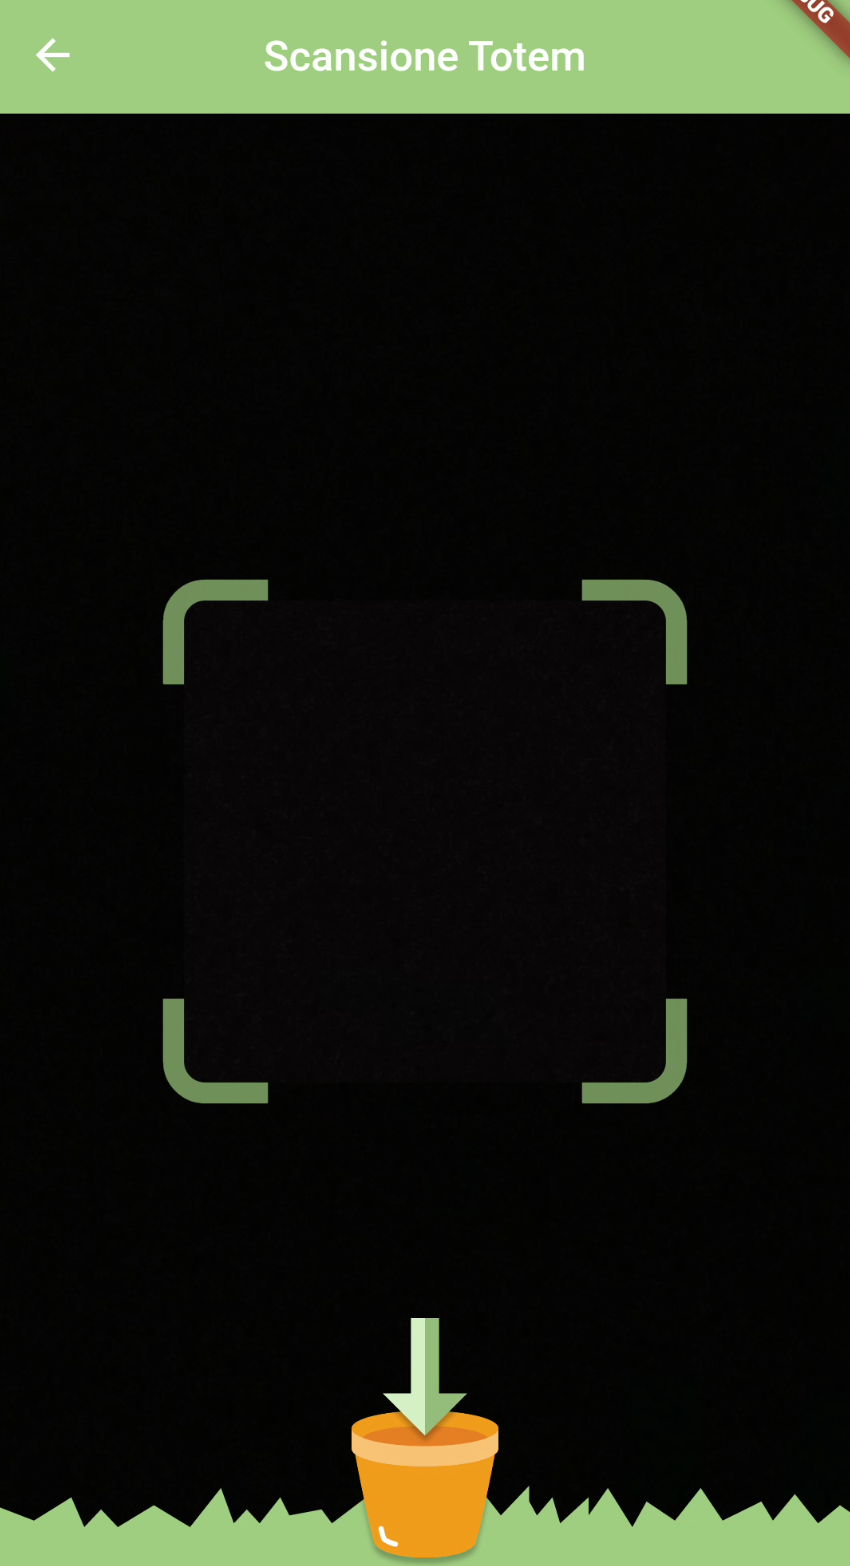
\includegraphics[width=0.3\textwidth]{img/app/uploadProgress.png}
        \label{fig:scanTotem}
    }
    \subfloat[Schermata di caricamento progressi]{
        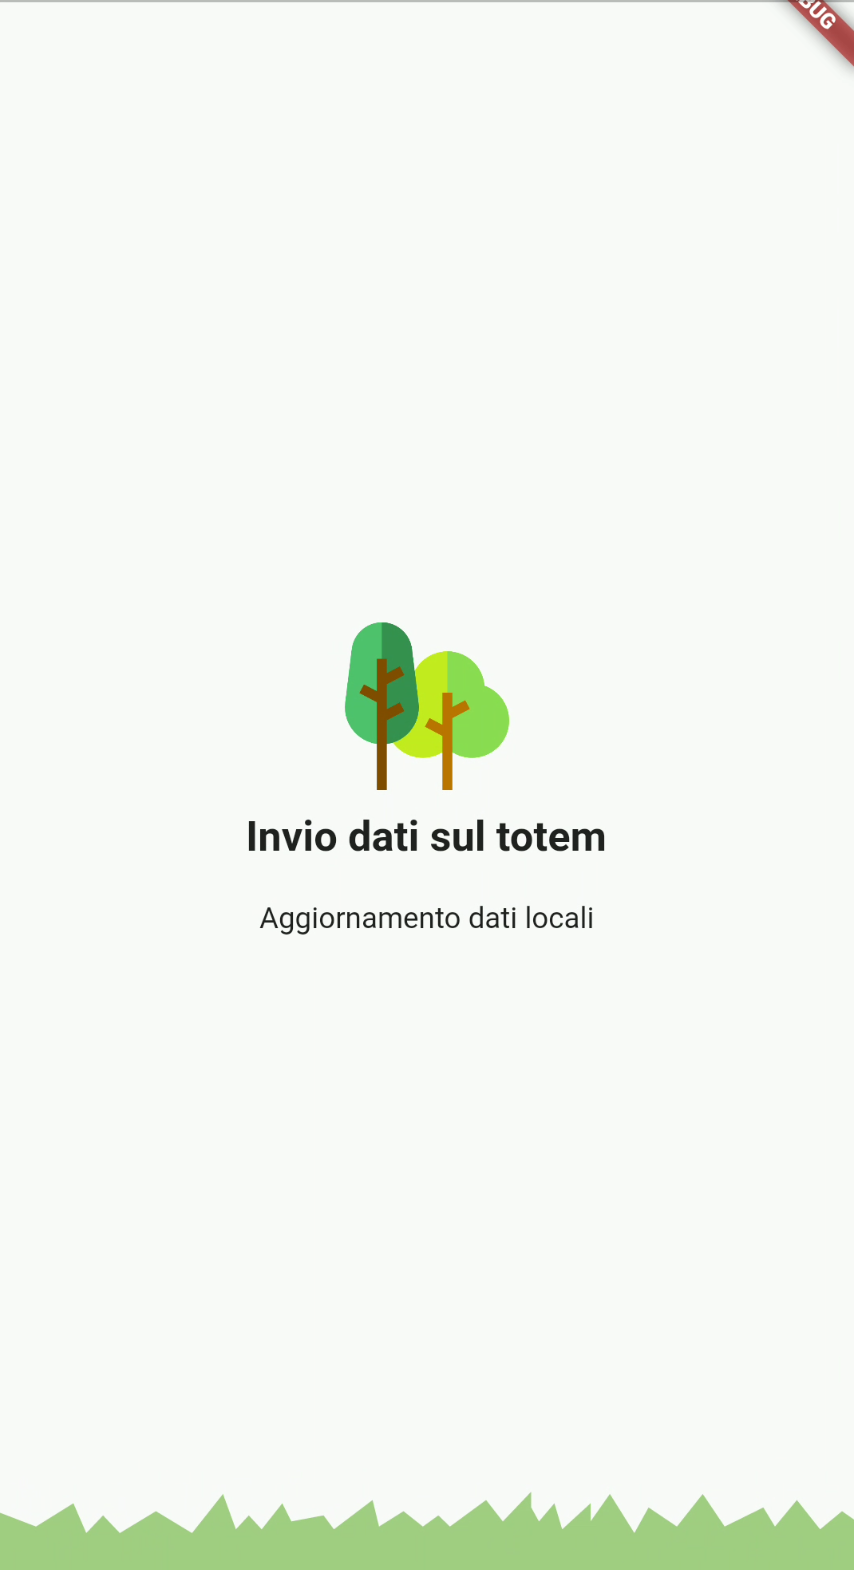
\includegraphics[width=0.3\textwidth]{img/app/uploadingPage.png}
        \label{fig:uploadinData}
    } 
    \caption{Screenshot schermate condivisione dati da app, scansione totem e caricamento}
    \label{fig:shareDataApp}
\end{figure}

\subsection{Pagina di condivisione progressi}
La schermata di caricamento dei progressi è raggiungibile dalla pagina utente oppure direttamente dalla pagina \textit{Home} in cui vi sono gli alberi collezionati. Nella barra degli strumenti (\texttt{AppBar}) di entrambe le pagine è stato aggiunto un pulsante (\texttt{IconButton})che permette di aprire la pagina di condivisione aggiungendola allo stack di schermate dell'app chiamando il metodo \textit{push} della classe \texttt{Navigator} che disciplina la navigazione fra pagine. Nel listato \ref{lst:shareIconButton} da riga 7 a riga 20 inclusa viene mostrato il codice inserito.

\begin{lstlisting}[style=FlutterStyle, caption={Codice aggiornato della barra degli strumenti dell'app: inserito pulsante per la condivisione dei progressi.}, label={lst:shareIconButton}]
    Scaffold (
      backgroundColor: Colors.white,
      appBar: AppBar(
        centerTitle: true,
        backgroundColor: mainColor, 
        title: const Text("Profilo"),
        leading: IconButton(
          onPressed: () => Navigator.push(
            context,
            MaterialPageRoute(builder: (context) {
              return const SharePorgressPage();
            }),
          ),
          icon: const Icon(
            Icons.upload,
            size: 25,
            semanticLabel: "Carica progressi",
          ),
        ),
      ),
      body: //contenuto della pagina Utente o della Home
    );
\end{lstlisting}

\subsection{Scansione QR e caricamento}
% Implementazione della schermata di scansione del qr del riutilizzo della schermata di scansione (forze pattern strategy), con schema d'interfaccia volendo 
% Implementazione della schermata con codice effettivo dell'implementazione del pattern mvi
\textcolor{red}{TODO: RIFORMULARE , IL CONCETTO è QUELLO}
La schermata della scansione del codice QR del totem prevede il riutilizzo della stesso componente utilizzato nella scansione del QR dell'albero. Infatti come si può vedere in figura ??, la schermata di scansione fa uso della classe \texttt{ScanQRView} che gestisce la fotocamera e la lettura dei codici QR. Riconosciuto un codice QR le informazioni contenute al suo interno vengono passate alla classe specifica per il totem che verifica la validità delle informazioni per poi procedere con la preparazione e caricamento dei progressi utente. Durante tutte le due fasi viene visualizzata la schermata in figura \ref{fig:uploadinData} che risulta reattiva in attesa di un esito del caricamento o della validità del codice QR.

Consiste specie di pattern strategy E in cui oltre la strategia che viene utilizzata per la validazione del codice QR scansionare si indica anche la schermata barra interfaccia utente che deve essere visualizzata dopo la scansione del codice. Ciò schermata poi possiede la sua strategia per validare ed utilizzare i dati presi dal QR.
\textcolor{red}{scegli se mettere solo future builder o tutta la classe}

 \begin{lstlisting}[style=FlutterStyle, caption={}, label={lst:strategyViewTotem}]
  Consumer<DataManager>(
    builder: (context, dataManager, child) => FutureBuilder<bool>(
      future: dataManager
          .uploadUserData(totemId)
          .timeout(const Duration(seconds: 8)),
      builder: (context, snap) {
        ConnectionState conState = snap.connectionState;
        bool uploadDone = snap.hasData ? snap.data! : false;
        if (conState == ConnectionState.waiting) {
          return const UploadingDataView();
        } else if (conState == ConnectionState.done) {
          if (uploadDone) {
            return const CompletedUploadView();
          } else {
            return const ErrorView(message: "Errore invio dati");
          }
        } else {
          return const ErrorView(message: "Errore sconosciuto");
        }
      },
    ),
  ),
\end{lstlisting}
%%%%%%%%%%%%%%%%%%%%% TOTEM %%%%%%%%%%%%%%%%%%%%%%%%%%%%%%%%
\section{Totem}
\subsection{Dati Firebase}
Una volta deciso di utilizzare il database Firebase Realtime, che è di tipo documentale, si è reso necessario convertire lo schema UML in figura \ref{fig:totemDomain} in formato JSON per avere la struttura generale dei dati che verranno memorizzati.
Per non avere troppi oggetti annidati, si è deciso di separare le informazioni del totem (listato \ref{lst:totemInfo}) dai dati utente che sono stati condivisi (listato \ref{lst:userDataTotem}).

\begin{lstlisting}[language=json, caption={Esempio di oggetto JSON contenente le informazioni sui totem}, label={lst:totemInfo}]
    "totemInfo": {
        "totemIdString": {
          "place": "locationName",
          "project": "projectName"
        },
      },
\end{lstlisting}  

\begin{lstlisting}[language=json, caption={Esempio di oggetto JSON che memorizza i dati utente per ciascun Totem}, label={lst:userDataTotem}]
      "totems": {
        "ces_remade": {
          "userNickname": {
            "badgeCount": 0,
            "co2": 0,
            "level": 0,
            "nickname": "userNickname",
            "paper": 0,
            "treesCount": 0
          }
        }
      }
\end{lstlisting}

\subsection{DataManager}
Il DataManager, come spiegato nel capitolo del design, funge sia da Repository che da Model del pattern MVI. Mantiene al suo interno i riferimenti ai diversi provider di cui fa uso, al momento solo \texttt{FirebaseProvider}, ed espone metodi che restituiscono \textit{State}, indirizzati alla \textit{View}, contenenti i dati utili alle schermate. A livello implementativo gli \textit{State} sono un oggetto della classe \texttt{Future} e vengono utilizzati come risultato ad una computazione asincrona permettendo di svolgerne altre finché non viene completata. Utilizzando \texttt{Future} come tipo di ritorno dei metodi del DataManager in combinazione con il \texttt{FutureBuilder} si individua una forma di pattern MVI con la possibilità di adattare la View in base allo stato della computazione.

La classe \texttt{DataManager}, come si può notare in riga 1 del listato \ref{lst:dataManager}, estende \texttt{ChangeNotifier} e questo permette di aggiornare la View con i nuovi dati aggiornati.
Inoltre viene utilizzato il pattern Observer sul FirebaseProvider: il DataManager, implementando l'interfaccia \texttt{FirebaseObserver} e aggiungendosi come observer (riga 8 listato \ref{lst:dataManager}), viene notificato per qualsiasi genere di modifica dei dati nel cloud.
In cascata quindi ogni modifica sul database Firebase fa scattare la notifica delle Views con il metodo \texttt{notifyListeners} (riga 24 listato \ref{lst:dataManager}).

\begin{lstlisting}[style=FlutterStyle, caption={Classe DataManager}, label={lst:dataManager}]
  class DataManager extends ChangeNotifier implements FirebaseObserver {
    final String _totemId = "ces_remade";
    late final FirebaseProvider _firebaseProvider;
  
    DataManager() {
      _firebaseProvider = FirebaseProvider(_totemId);
      _firebaseProvider.addObserver(this);
    }
  
    String getCurrentTotemId() {
      return _totemId;
    }
  
    Future<List<SharedData>> getData() async {
      return _firebaseProvider.getTotemData();
    }
  
    Future<List<SharedData?>> getTop10User() async {...}
  
    Future<Map<StatId, String>> getStatistics() async {...}
  
    @override
    void firebaseNotify() {
      notifyListeners(); 
    }
  }
\end{lstlisting}

\subsection{Pagina Home} 
Per la pagina principale è stata sviluppata l'idea del mockup in figura \ref{fig:forestHome} dove vengono visualizzate le chiome degli utenti che insieme compongono un bosco rigoglioso ed è stato scelto questo design grafico in quanto più affine all'idea di bosco virtuale. Con una visualizzazione di questo genere gli utenti hanno una maggiore percezione del senso di comunità dove ciascun giocatore contribuisce a rendere il bosco più verde e ricco di alberi. In figura \ref{fig:homepage} viene mostrata una istantanea della homepage mentre nel listato \ref{lst:homepageCode} è possibile consultare il codice che si occupa della disposizione degli alberi e del loro comportamento al tocco dove rispettivamente è stato utilizzato il widget \texttt{GridView} (riga 8) e la classi \texttt{GestureDetector} (riga 14).

Per questa pagina, come per le altre che seguono, è stato utilizzato sempre la stessa metodologia e architettura del codice per la loro creazione: con l'ausilio del \texttt{FutureBuilder} è stato possibile gestire con maggiore semplicità ed astrazione il pattern MVI. 
\textcolor{red}{CONTROLLA sotto}
Più precisamente all'atto della creazione dell View vengono richiesti i dati al \texttt{DataManager} chiamando il metodo specifico che soddisfa l'intent. Il datamanager quindi restituisce un tipo di dato future<List<SharedData>> (State) che permette di avere una interfaccia reattiva nonostante l'intent dell'utente debba essere ancora evaso.

\begin{figure}[h]
  \centering
  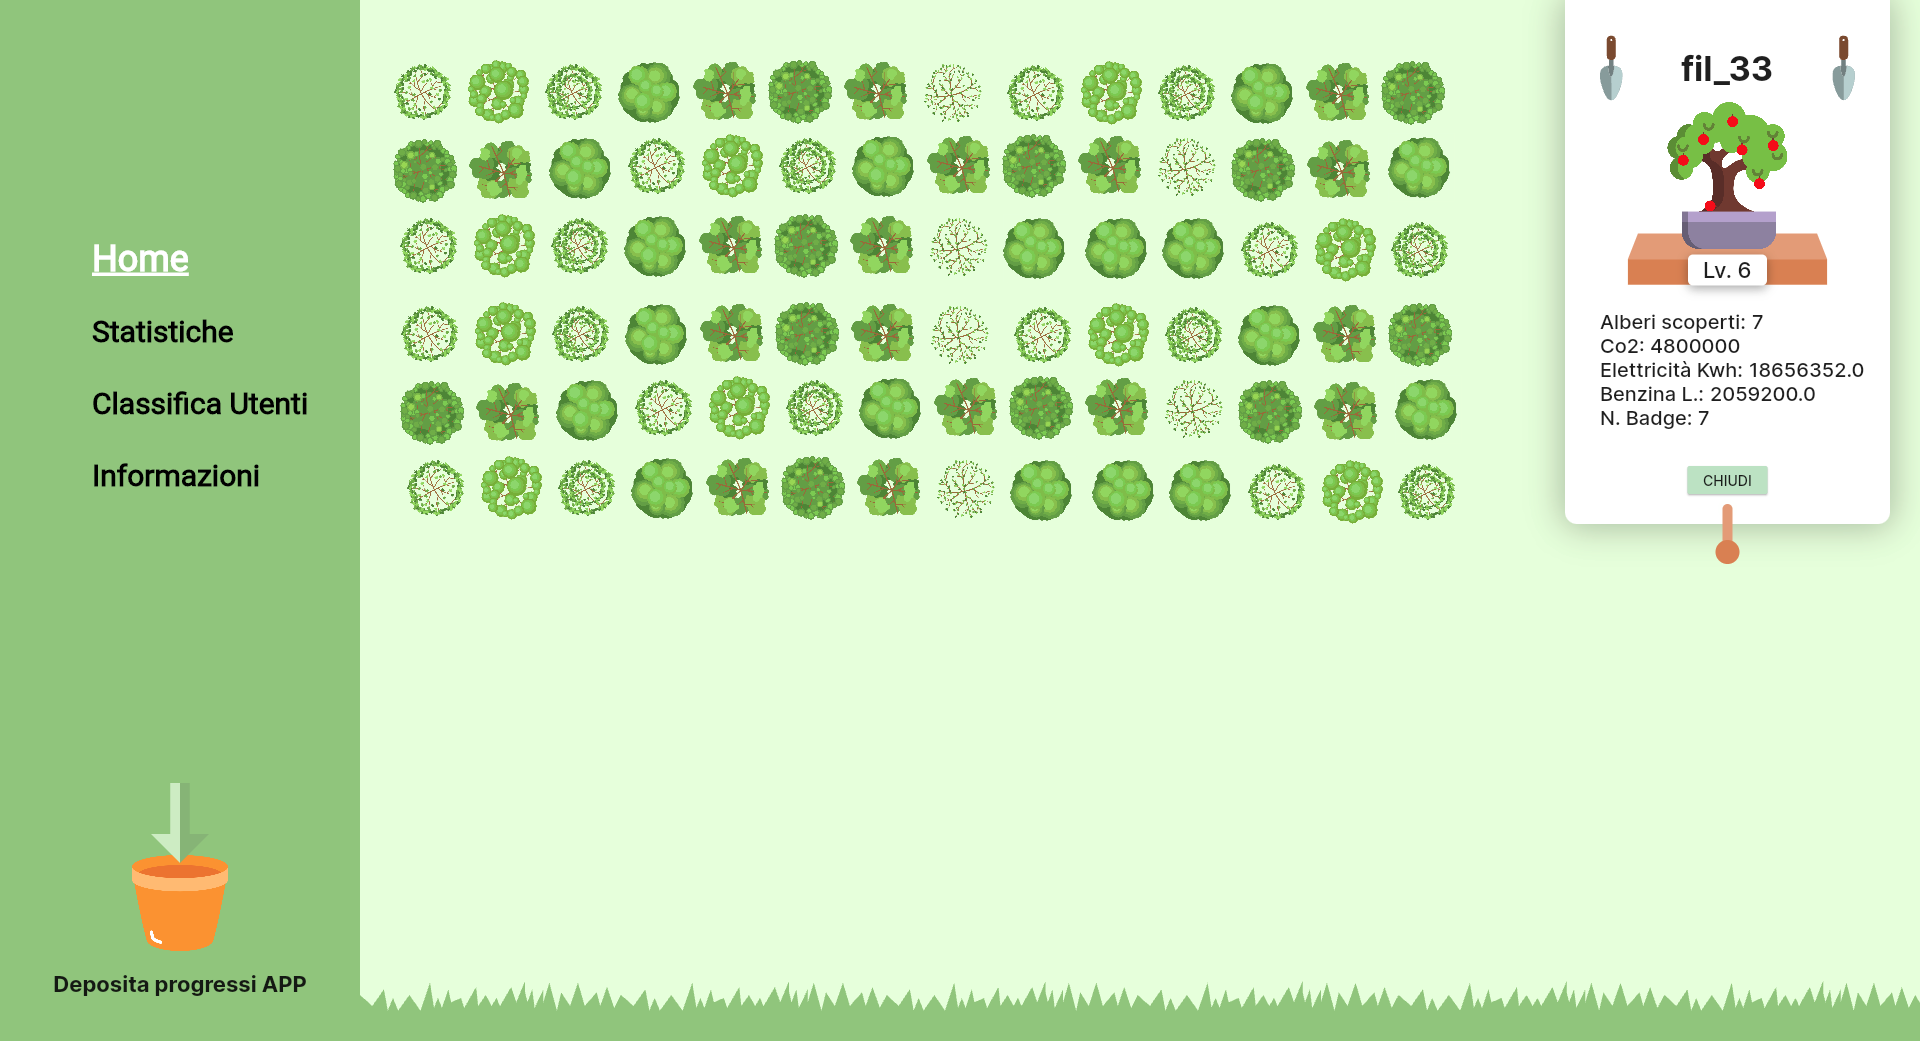
\includegraphics[width=\textwidth]{img/totem/screenshot/homepage.png}
  \caption{Screenshot della pagina Home dove viene visualizzato il bosco virtuale costruito dalla partecipazione degli utenti.}
  \label{fig:homepage}
\end{figure}
\newpage
\begin{lstlisting}[style=FlutterStyle, caption={Parte del codice per la creazione del bosco della Homepage}, label={lst:homepageCode}]
Consumer<DataManager>(
builder: (context, dataManager, child) =>
    FutureBuilder<List<SharedData>>(
    future: dataManager.getData(),
    builder: (context, snapshot) {
      if (snapshot.hasData) {
        // widget per la disposizione a griglia delle chiome
        return GridView.count(
          crossAxisCount: 20,
          mainAxisSpacing: 10,
          crossAxisSpacing: 10,
          children: (snapshot.data ?? []).map(
            (userDataTree) {
              return GestureDetector(
                onTap: () {
                  setState(() {
                    userData = userDataTree;
                    showDetails = !showDetails;
                  });
                },
                // chioma dell'albero dell'utente
                child: ForestTree(level: userDataTree.level),
              );
            },
          ).toList(),
        );
      } else {
        return const Center(
            child: CircularProgressIndicator(
          color: Color.fromRGBO(161, 204, 130, 1),
        ));
      }
    },
  ),
),
\end{lstlisting}
%
%
\subsection{Pagina Statistiche}
% Animazione dell'elemento della griglia, creazione della pagina, quali widget flutter sono stati utilizzati per il caricamento dei dati e la loro attesa, operazioni che vengono svolte all'interno di data manager per ricavare i dati, i cerchi alla fine sono tutti colorati non sono indicatori gauge come si era pensato 

%
%
\subsection{Classifica}
Schermata della classifica, le modifiche grafiche che ha subito, l'aggiunta dell'alberello e info di co2, caricamento dati solito pattern mvi, come viene stilata la classifica codice lato repository (datamanager)... Ipotesi di poter decidere su cosa viene fatta la classifica es. co2, benzina o che altro. anche se poi alla fine le quantità sono proporzionali, cambierebbe poco la classifica.


\begin{figure}[h]
  \centering
  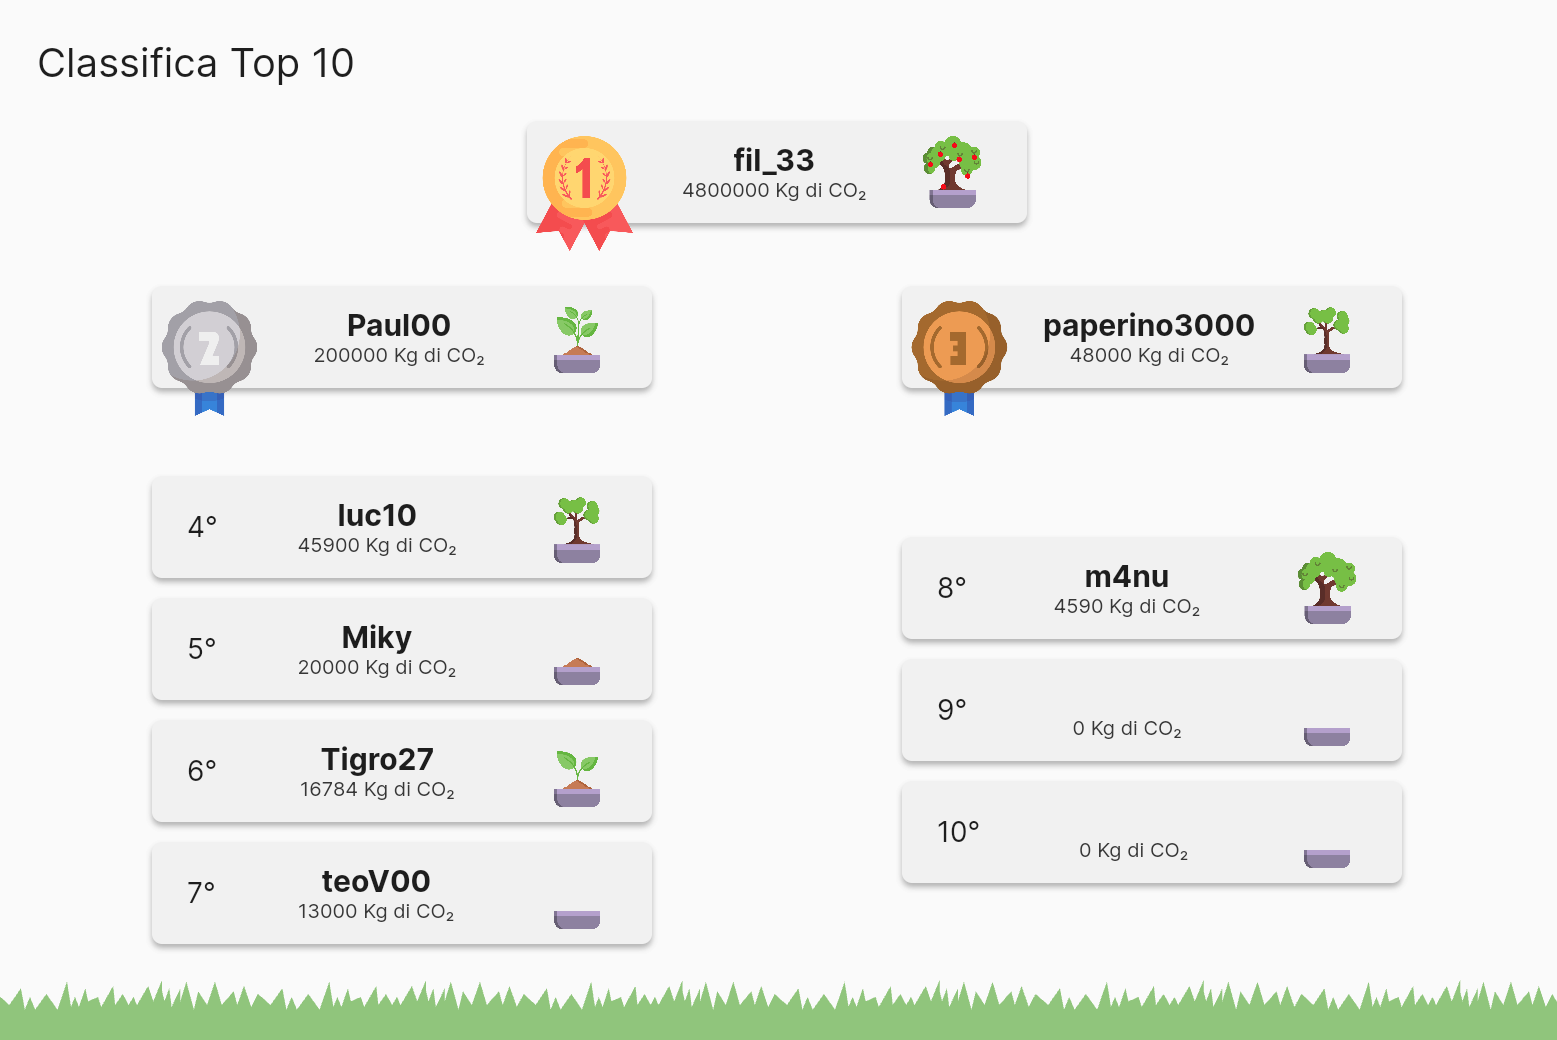
\includegraphics[width=\textwidth]{img/totem/screenshot/top10screen.png}
  \caption{Pagina della classifica conclusa.}
  \label{fig:top10screen}
\end{figure}

%
%
\subsection{Pagina Informazioni}
% Pagina informazioni, struttura a griglia, le classi che sono state create e politica di disposizione delle tiles;  pattern observer per mostrare e chiudere il pop up delle info
% come si deve fare per aggiungere una tile e impostazioni delle tile, grandezza e contenuto
La pagina delle informazioni nel corso del suo concepimento ha subito vari cambiamenti, come anche indicato nel capitolo Design \ref{subsec:totem} in cui viene trattato il design del totem, che comprendono un cambio drastico di layout passando da una semplice pagina scorrevole ad uno a visualizzazione a griglia; la decisione d'implementare quest'ultimo è stata molto condizionata dall'esito di un sondaggio eseguito su un piccolo gruppo di utenti target, che provando entrambi i mockup su device touchscreen, hanno dimostrato una maggiore preferenza per la visualizzazione a piastrelle (\textit{tiles}) in quanto più immediata, ordinata e di facile comprensione, prediligendo il tipo d'interazione \enquote*{a tocco} (\textit{tap gesture}) con l'interfaccia per accedere alle informazioni al posto dello scorrimento verticale (\textit{vertical scrolling gesture}). In figura \ref{fig:infoPage} viene mostrata la pagina delle informazioni ottenuta mentre in figura \ref{fig:infoPagePopup} è possibile vedere come, dopo il tocco di una tile, vengono mostrate le informazioni dettagliate.

\begin{figure}[h]
  \centering
  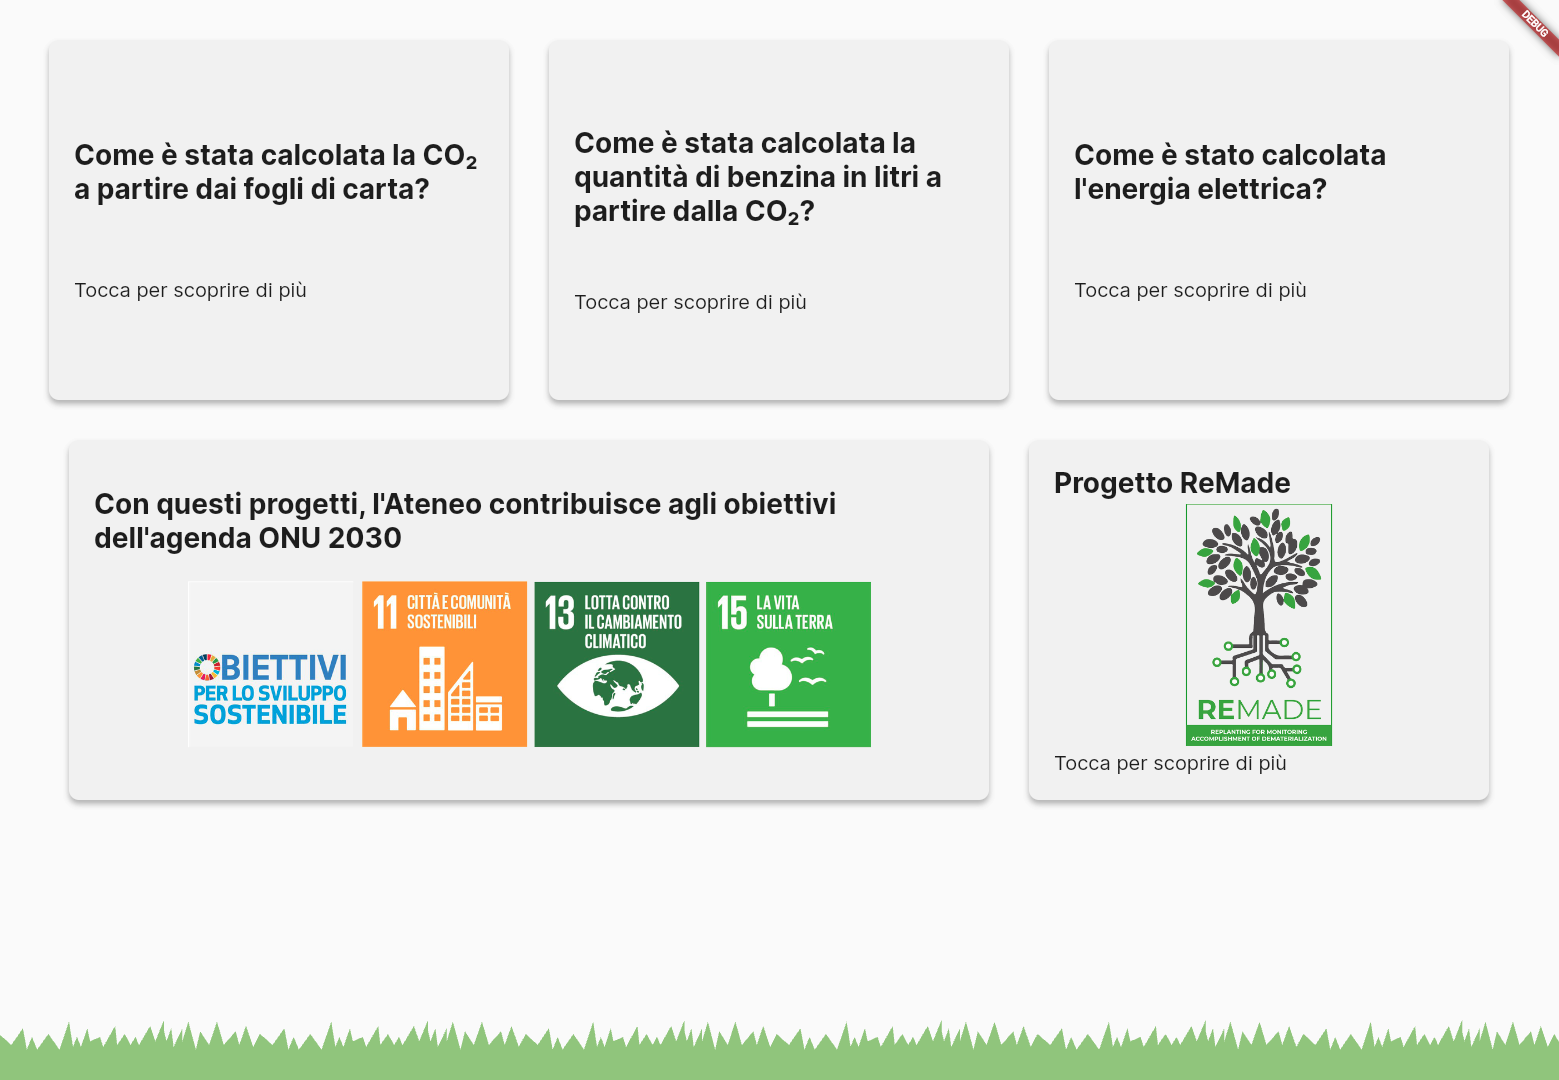
\includegraphics[width=\textwidth]{img/totem/screenshot/infoPageScreen.png}
  \caption{Pagina delle informazioni effettiva}
  \label{fig:infoPage}
\end{figure}
\begin{figure}[h]
  \centering
  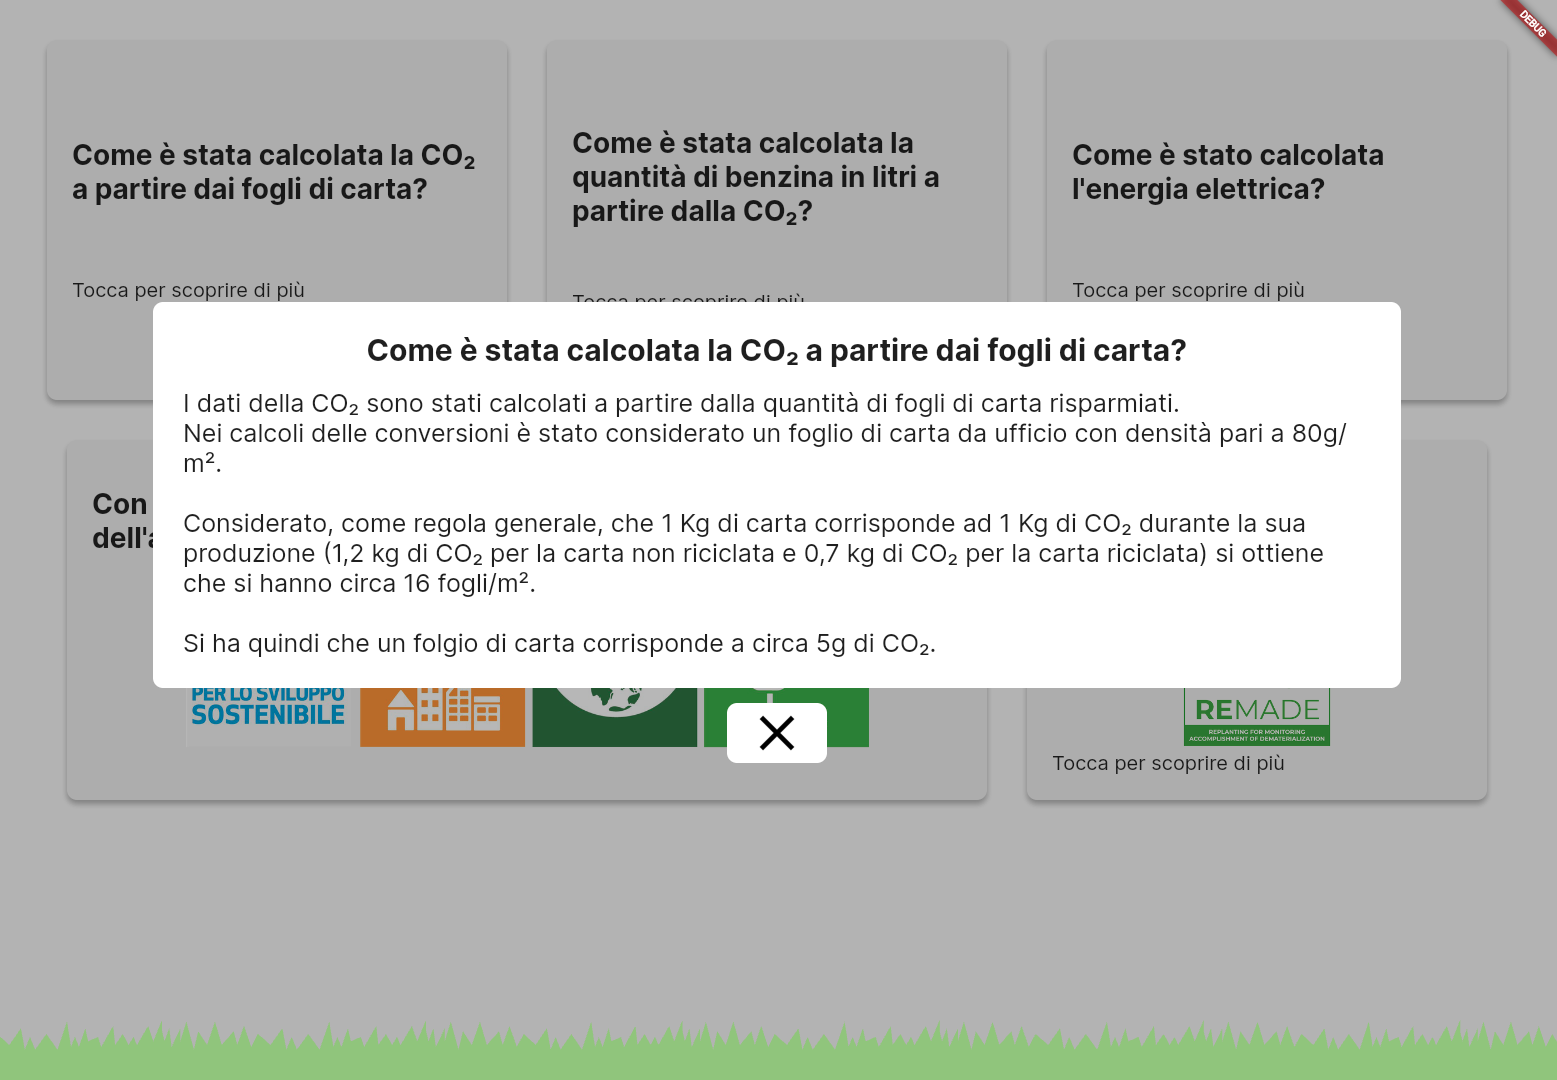
\includegraphics[width=\textwidth]{img/totem/screenshot/infoPagePopupScreen.png}
  \caption{Pagina delle informazioni: vengono mostrati i dettagli relativi alla tile cliccata.}
  \label{fig:infoPagePopup}
\end{figure}

Per la composizione della vista a griglia è stato utilizzato il widget \texttt{GridView} utilizzando un layout personalizzato definito dalla classe \texttt{SliverQuiltedGridDelegate} del package flutter \texttt{flutter\_staggered\_grid\_view} \cite{staggeredGridView} che permette di mostrare elementi che possono occupare più di una cella e colonna.

% \begin{figure}[h]
%   \centering
%   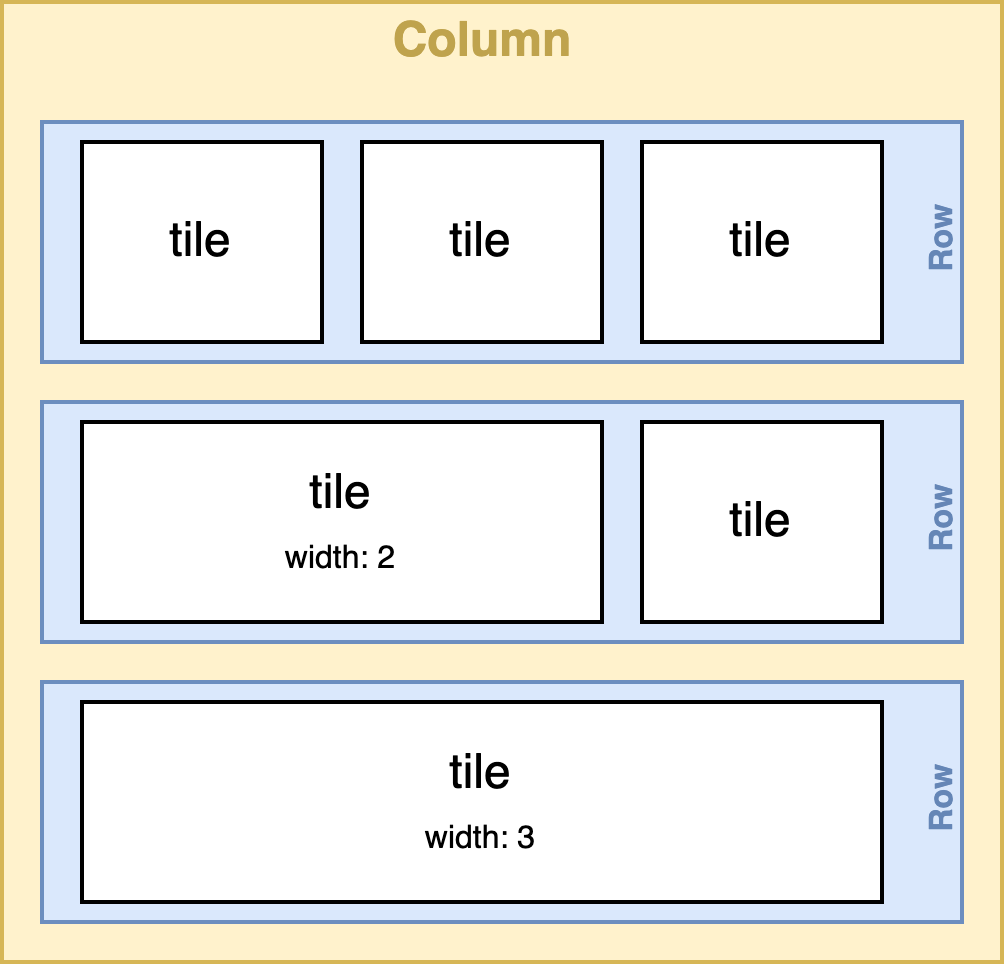
\includegraphics[width=8cm]{img/totem/infopage-layout.png}
%   \caption[Layout pagina informazioni]{Layout della pagina delle informazioni del totem considerando una larghezza di 3 colonne}
%   \label{fig:infopageLayout}
% \end{figure}

% \begin{lstlisting}[language=pseudocode, caption={Pseudocodice per la costruzione della griglia di Tiles con occupazione della riga variabile}, label={lst:gridTileViewClass}]
% rowsAmount = tilesToPlace / itemsPerRow
% for row = 0 to rowsAmount
%   while rowCapacity > 0 and tilesToPlace list not empty
%     if row can contain tile
%       add tile to row
%       remove tile from tilesToPlace list
%     else 
%       skip to next tile in tilesToPlace list

%   create row graphic-element

% return column view with previous rows
% \end{lstlisting}

\section{Testing e Debug}
